\section{Teilaufgabe 16}
\begin{aufgabe}
    Berechnen Sie mit dem Laplace Endwertsatz die stationäre Regeldifferenz 
    (im Prozent) für eine konstante Referenzdrehzahl (der Lastmoment ist 
    gleich null).  Das Ergebnis ist eine Funktion von $K_p$ . Prüfen Sie Ihr 
    Ergebnis mit dem im Simulink programmierten Regelkreis (Testen Sie mehrere 
    Werte für $K_p$ ).
\end{aufgabe}
\[ E(s) = 1 - G_F(s) 
    = 1 - \frac{K_p \cdot K_g}{\tau \cdot s + 1 + K_p \cdot K_g}
\]
\[ e(t \to \infty) = \lim\limits_{s \to 0} E(s) \]
\[ \lim\limits_{s \to 0} E(s)
    = 1 - \lim\limits_{s \to 0}
        \left(\frac{K_p \cdot K_g}{\tau \cdot s + 1 + K_p \cdot K_g}\right)
    = 1 - \frac{K_p \cdot K_g}{1 + K_p \cdot K_g}
    = 1 - \left(1 - \frac{1}{1 + K_p \cdot K_g}\right)
    = \frac{1}{1 + K_p \cdot K_g}
\]
\begin{figure}[h!]
    \centering
    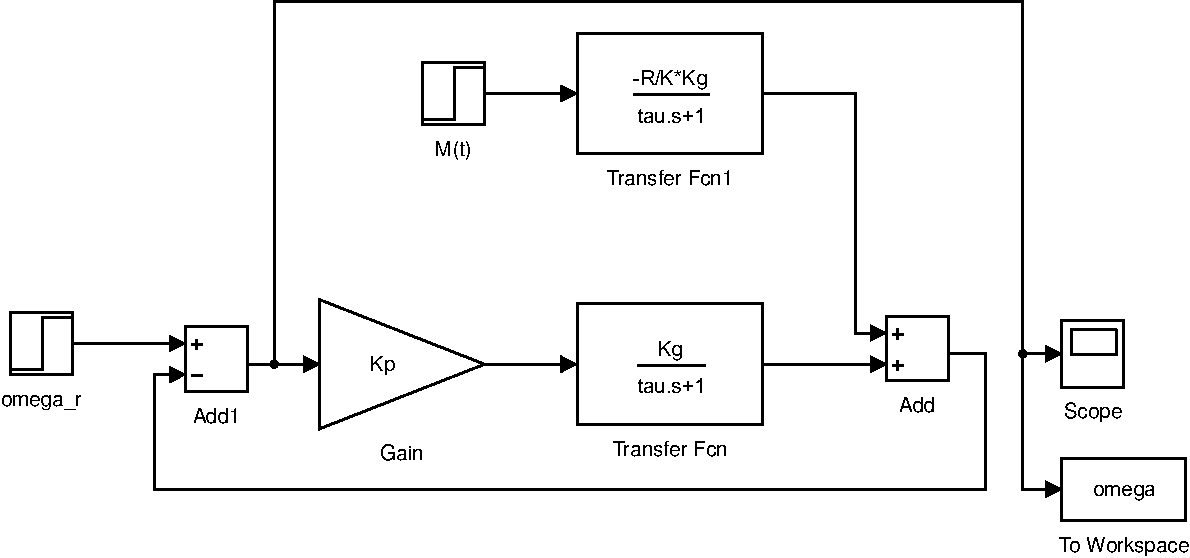
\includegraphics[width=0.6\textwidth]{16/regler_diff.pdf}
    \caption{Regler in Simulink}
    \label{fig:15}
\end{figure}
\begin{figure}[h!]
    \centering
    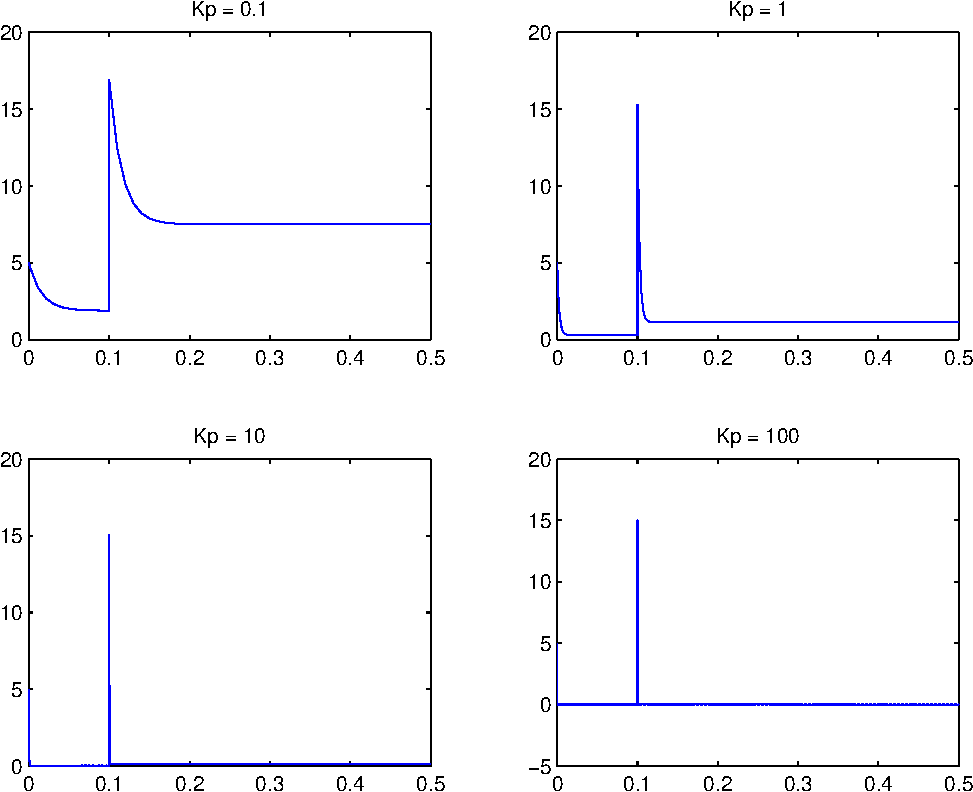
\includegraphics[width=0.6\textwidth]{16/regler_diff_plot.pdf}
    \caption{Simulationsergebnis}
    \label{fig:15plot}
\end{figure}
\begin{table}[h!]
    \centering
    \begin{zebratabular}{ll}
        \rowcolor{gray}
        $K_p$   & $e(t \to \infty)$ \\
        0.1     & 0.3750 \\
        1       & 0.0566 \\
        10      & 0.00596 \\
        100     & 0.00059964 \\
    \end{zebratabular}
\end{table}
\lstinputlisting{16/regler_diff.m}
